\documentclass{article}

\usepackage{fancyhdr}
\usepackage[includeheadfoot,left=1in, right=0.5in, top=0.5in, bottom=0.5in]{geometry}
\usepackage{lastpage}
\usepackage{extramarks}
\usepackage[usenames,dvipsnames]{color}
\usepackage{graphicx}
\usepackage{listings}
\usepackage{courier}
\usepackage{tikz}
\usepackage{color}
\usepackage{float}
\usepackage{url}
\usepackage{subfigure}
\usepackage{varwidth}
\usepackage{caption}
\usepackage{multirow}
\usepackage[pdfborder={0 0 0}]{hyperref}
\usepackage[compact,small]{titlesec}
\usepackage{microtype}
\usepackage{verbatim}
\usepackage{booktabs}
\usepackage{indentfirst}

\parskip = 0.5\baselineskip
\setlength{\belowcaptionskip}{-\baselineskip}

\captionsetup{font=scriptsize}
\captionsetup{labelfont=bf}

\pagestyle{fancy}
\rhead{Max Thrun \& Xiaohui Qi}
\lhead{EECE6080 - HW 3}
\rfoot{Page\ \thepage\ of \protect\pageref{LastPage}}
\cfoot{}
\renewcommand\headrulewidth{0.4pt}
\renewcommand\footrulewidth{0.4pt}

% make verbatim text small
\makeatletter
\g@addto@macro\@verbatim\small
\makeatother

\setlength\parindent{0pt} % Removes all indentation from paragraphs

\definecolor{sh_comment}{rgb}{0.12, 0.38, 0.18 } %adjusted, in Eclipse: {0.25, 0.42, 0.30 } = #3F6A4D
\definecolor{sh_keyword}{rgb}{0.37, 0.08, 0.25}  % #5F1441
\definecolor{sh_string}{rgb}{0.06, 0.10, 0.98} % #101AF9

\lstset{
    language=vhdl,
    xleftmargin=.25in,
    xrightmargin=.25in,
    numbers=left,
    numberstyle=\tiny,
    frame=tb,
    showstringspaces=false,
    captionpos=b,
    stringstyle=\color{sh_string},
    keywordstyle = \color{sh_keyword}\bfseries,
    commentstyle=\color{sh_comment}\itshape,
    basicstyle=\small\sffamily,
    %numbersep=-5pt,
    belowskip=\baselineskip,
    aboveskip=\baselineskip
}

\title{
    \vspace{2in}
    \textmd{\textbf{EECE6080 - HW 3}}\\
    \vspace{4in}
}
\author{\textbf{Max Thrun \& Xiaohui Qi}}

\begin{document}
\maketitle
\newpage
\subsection*{Part 1}

The objective of this part was to write a VHDL model of a parameterized n-bit
FUN generator which accepts a generic parameter \texttt{n} and
two n-bit vectors. The VHDL model we came up with is shown below:

\lstinputlisting[caption=Generic n-bit FUN generator]{../part_1/fun.vhd}

In order to test the functionality of our module we decided on an exhaustive
test that checked every possible input. Given the small size of the design this
was a reasonable approach as the execution time was negligible and it proved
100\% correct functionality in the design. By using \texttt{assert} statements
to check the output of the FUN module for each input condition the test is
completely automated.  The testbench used to drive the simulation is shown
below. Note that the same testbench was used for both 3 and 8 bit-widths with
the only change being the constant \texttt{n}.

\lstinputlisting[caption=FUN Testbench, label=funtb]{../part_1/fun_3_tb.vhd}

\newpage
While our testbench is exhaustive and reported no failures we still spot
checked the waveforms to ensure it was working as expected. The two screenshots
below show that each configuration is performing as expected with the correct
functionality.

\vspace{0.25in}
\begin{figure}[H]
    \centering
    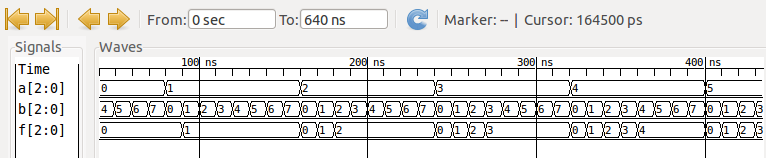
\includegraphics[width=\linewidth]{../part_1/fun_3.png}
    \caption{3-Bit FUN Generator Simulation Waveform}
\end{figure}
\vspace{0.25in}
\begin{figure}[H]
    \centering
    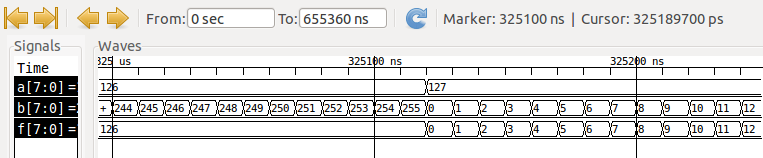
\includegraphics[width=\linewidth]{../part_1/fun_8.png}
    \caption{8-Bit FUN Generator Simulation Waveform}
\end{figure}

\newpage
\subsection*{Part 2}

The objective of this part was to redesign the FUN module to utilize 1-bit
slices. In order to do this we first came up with a slice design which we think
is fairly optimized. It is composed of two main parts: a magnitude comparator,
and a 2:1 multiplexer. The idea is that you can chain the magnitude comparators
together and loop back the output of the last comparator to the select lines of
each mux. A schematic representation of this design is shown below.

\begin{figure}[H]
    \centering
    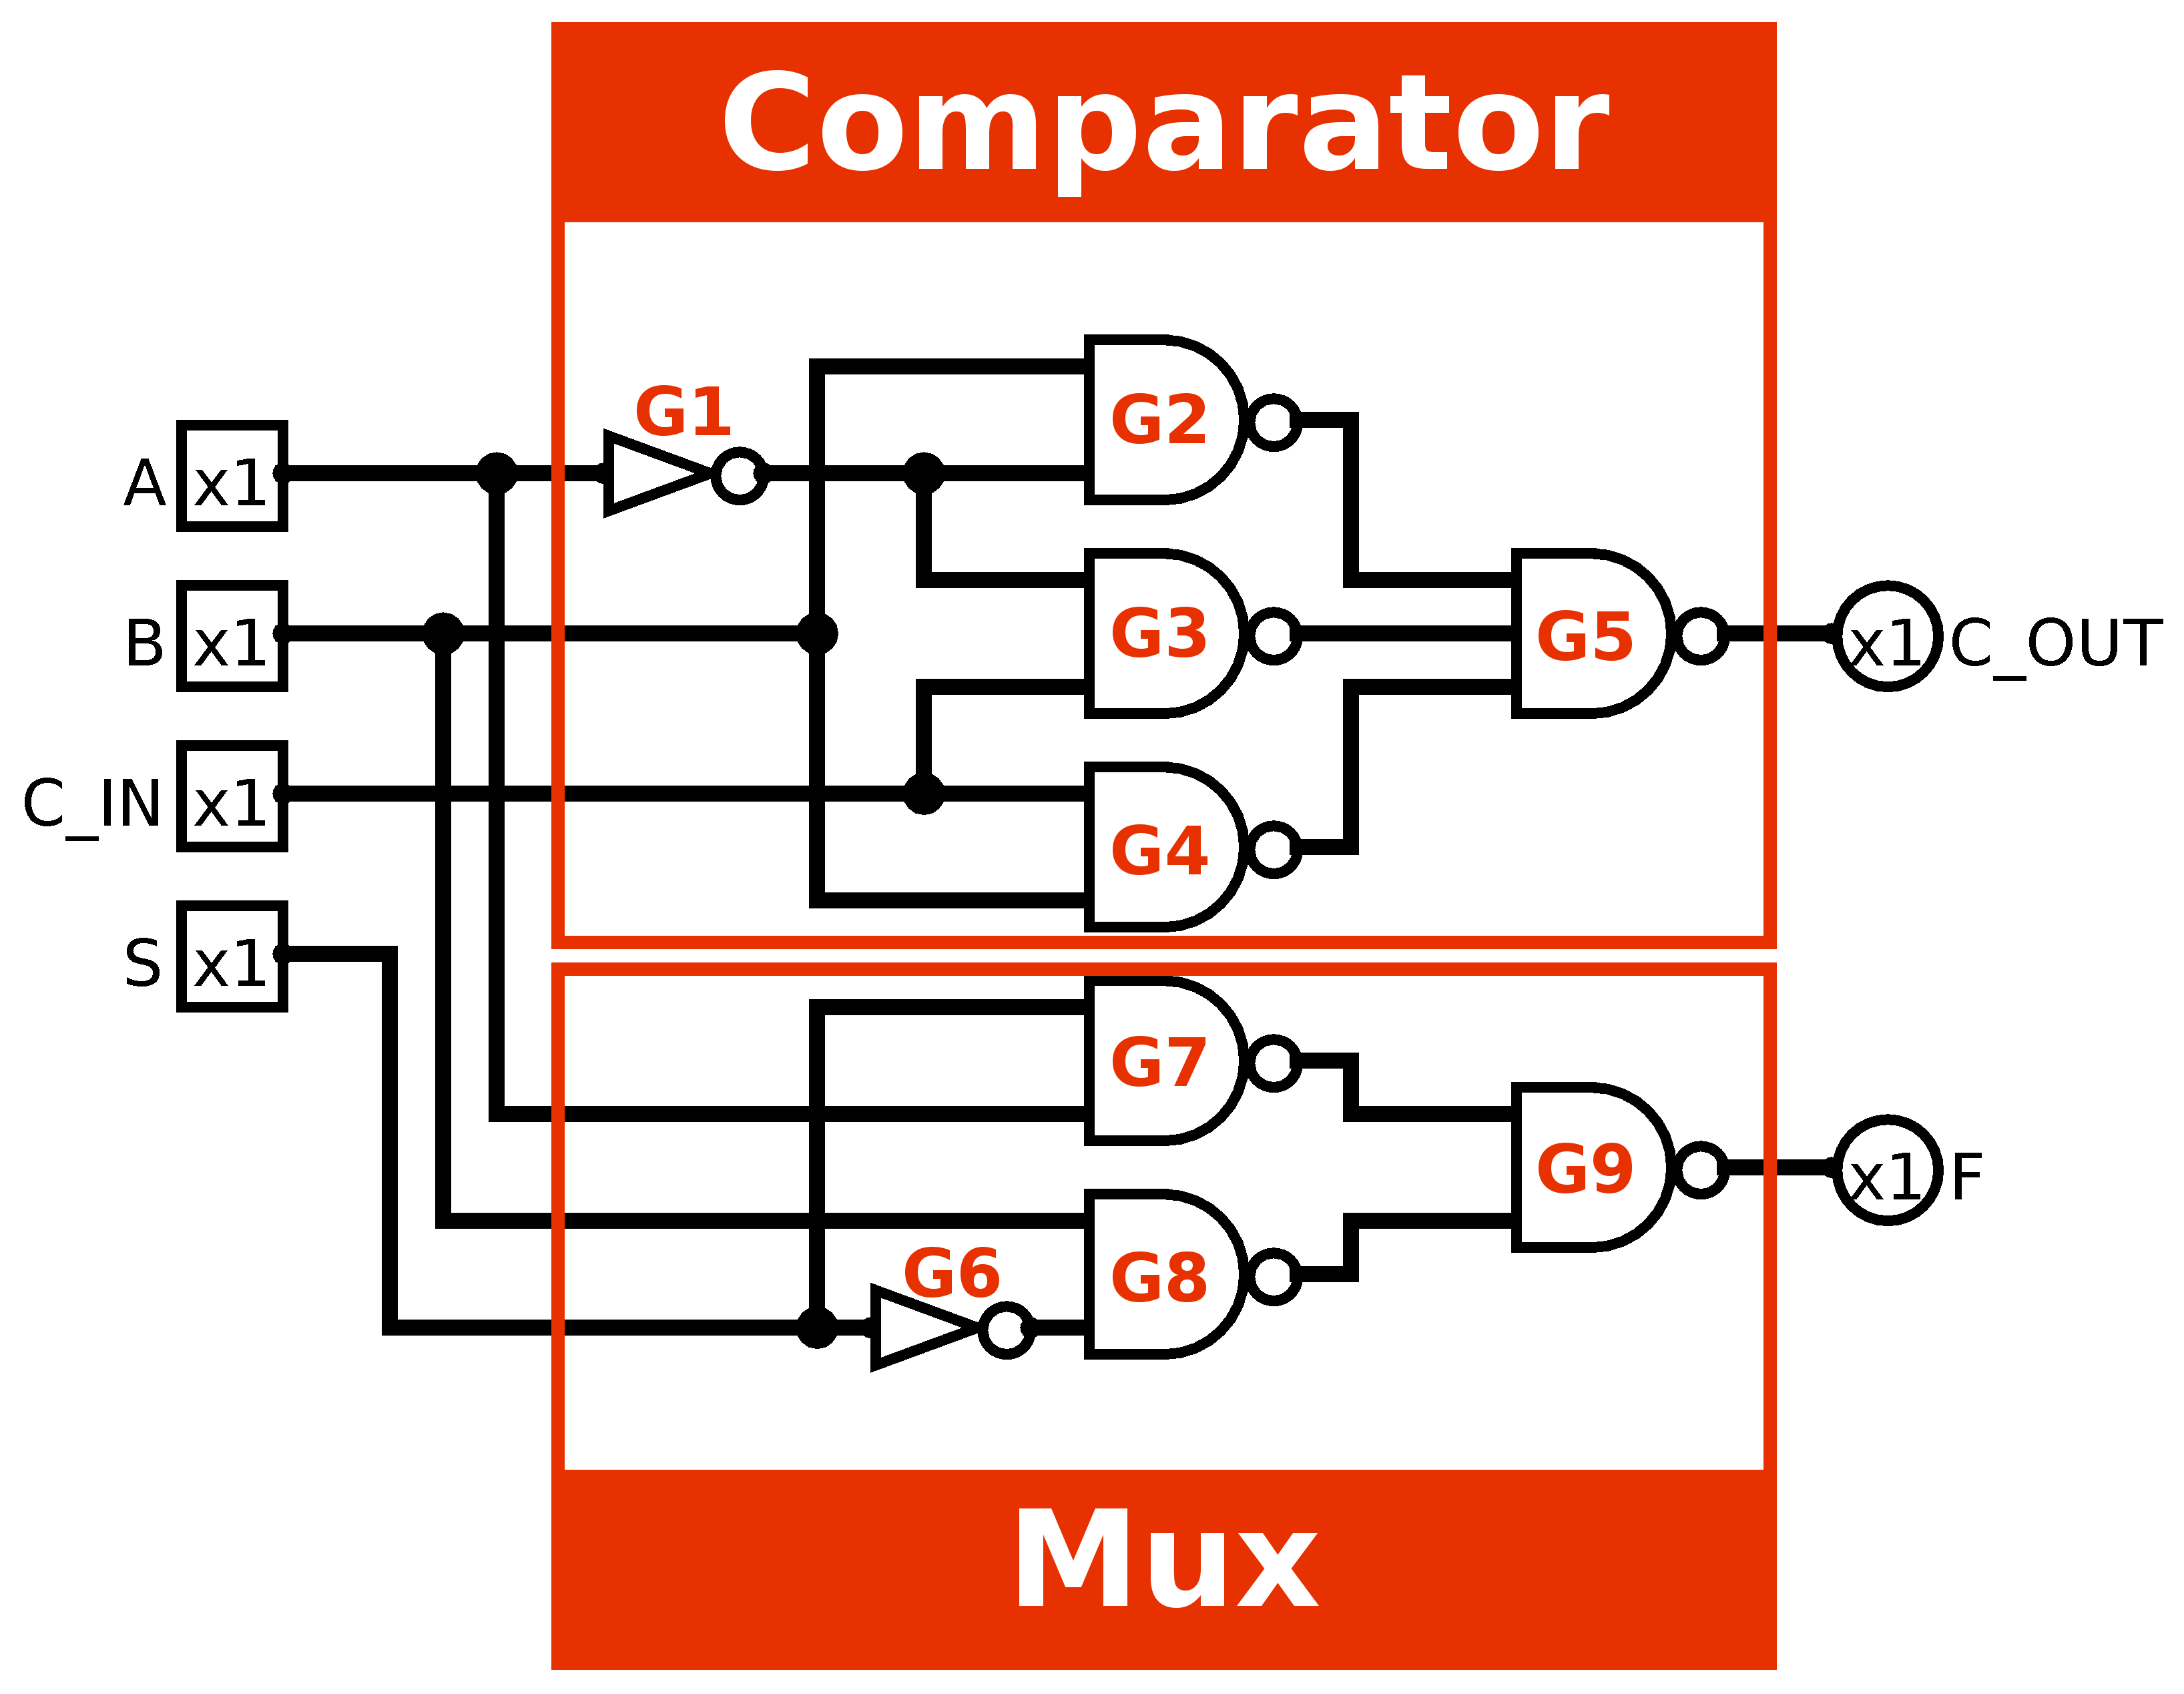
\includegraphics[width=0.75\linewidth]{../logisim/logisim_bitslice_gates_labeled.png}
    \caption{Gate Level Slice}
\end{figure}

An example circuit showing 4 slices chained together is shown below to
illustrate the connections.

\begin{figure}[H]
    \centering
    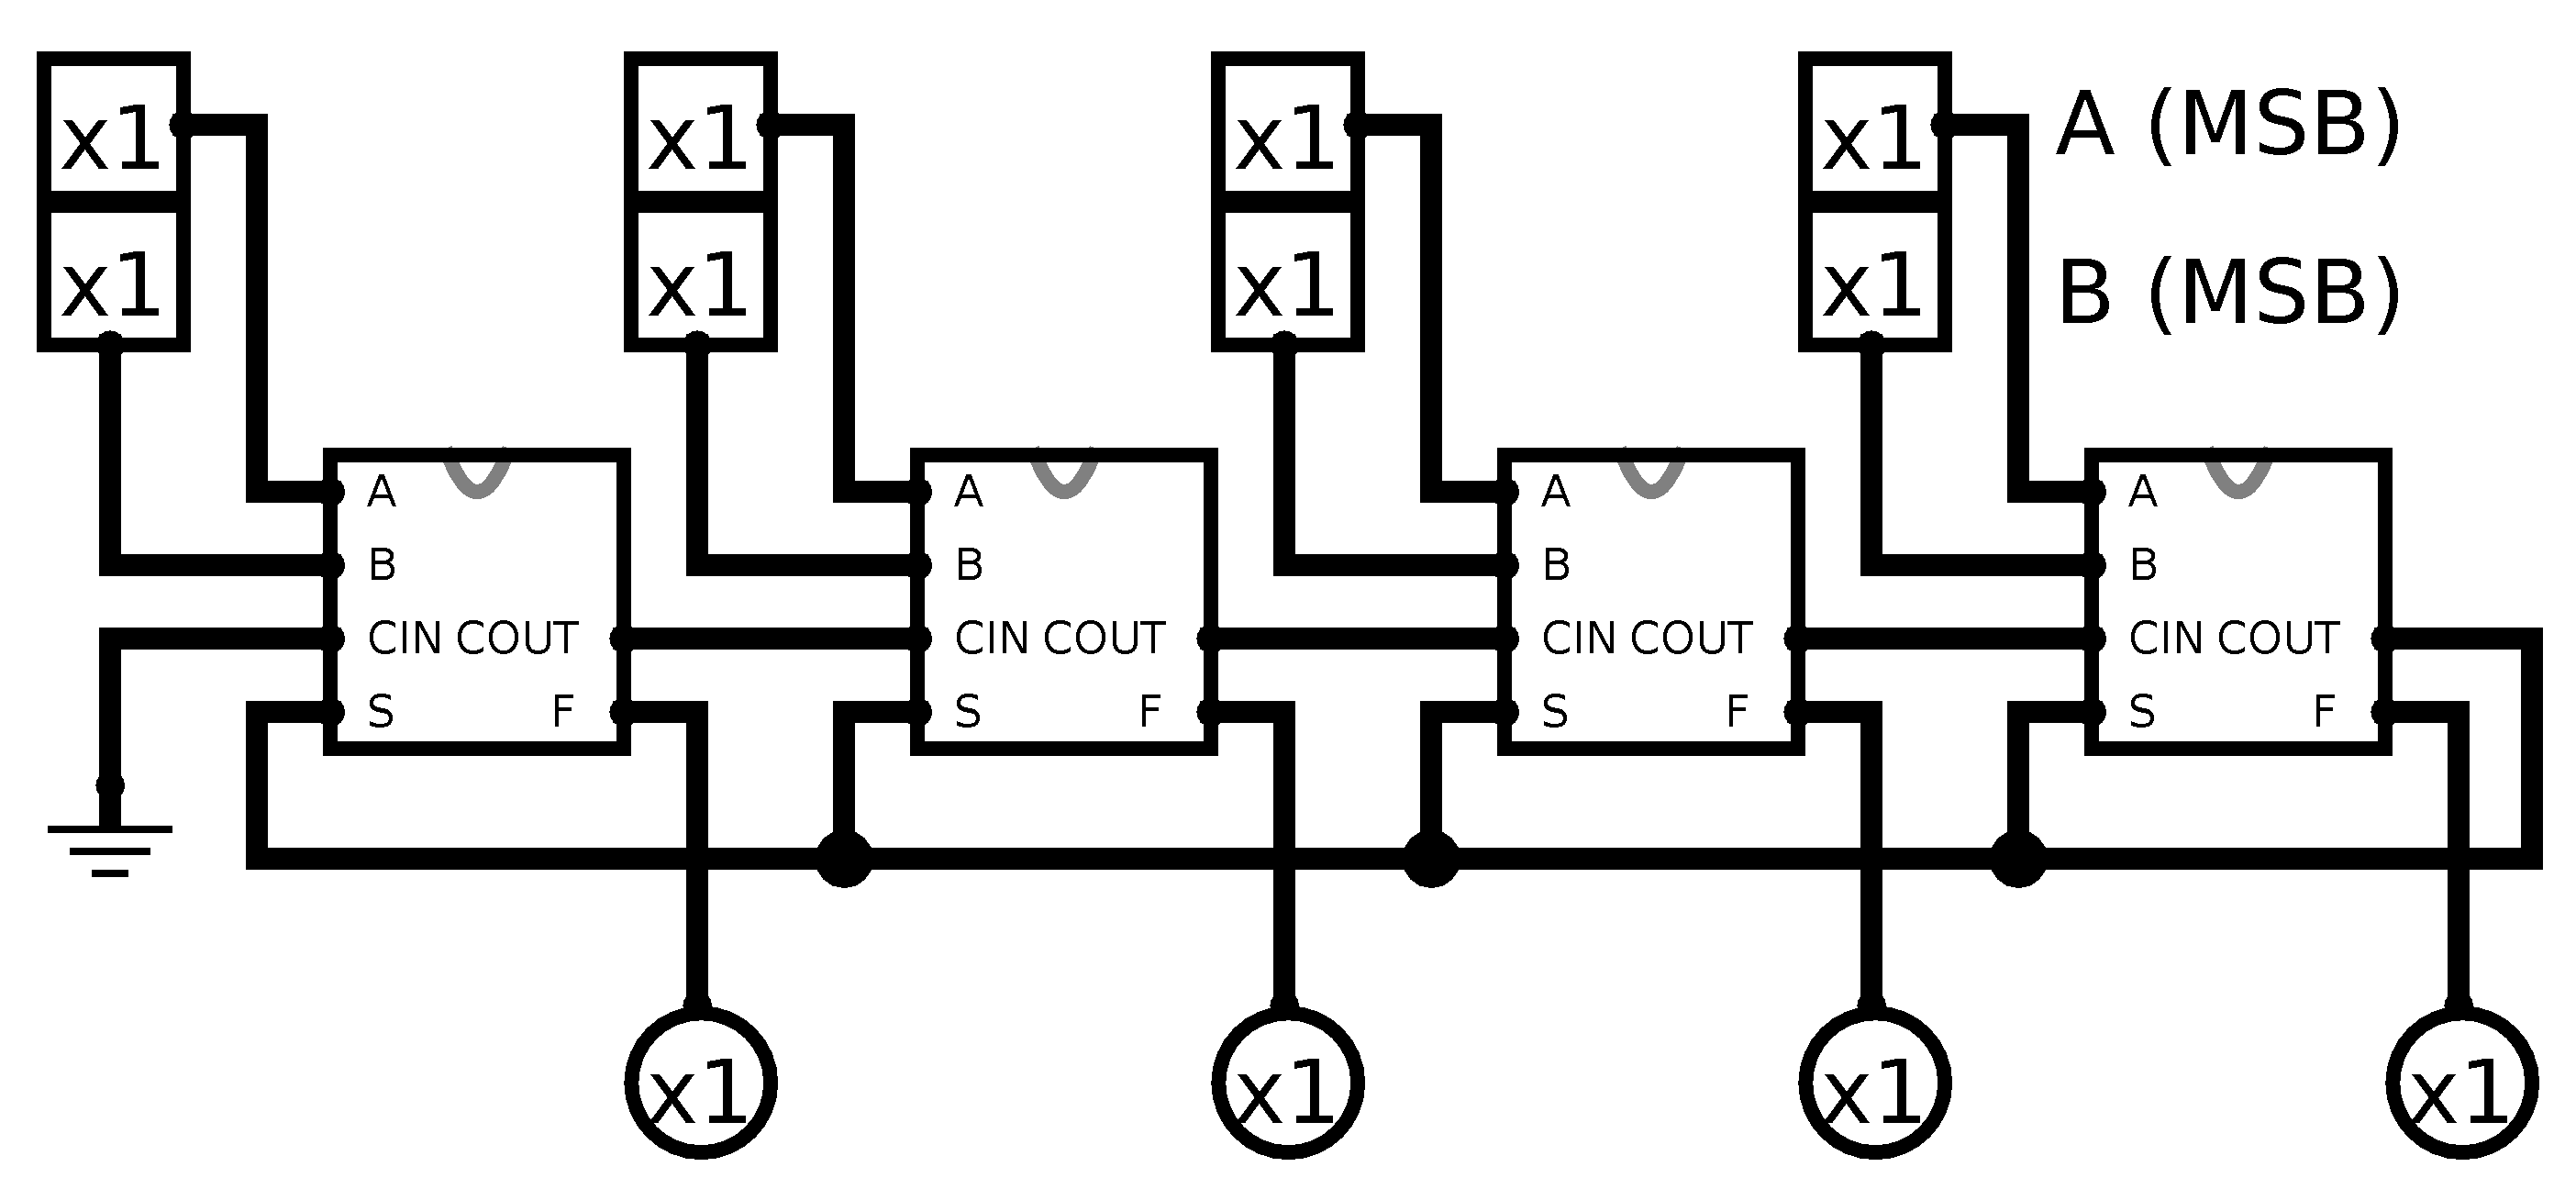
\includegraphics[width=0.75\linewidth]{../logisim/logisim_main.png}
    \caption{4 Slice Chain}
\end{figure}

\newpage
With the slice designed we translated it into a behavioral VHDL module shown below.

\lstinputlisting[caption=Single Slice]{../part_2/slice.vhd}

We then transformed the FUN module to use \texttt{generate} in order to
automatically chain \texttt{n} slices together. The FUN module is fairly simple
with just a single generate block and a vector to hold the carries between
slices.

\lstinputlisting[caption=FUN module using `generate']{../part_2/fun.vhd}

In order to ensure that the \texttt{generate} block was mapping the slices
correctly we synthesized a 3-bit version of our design in Quartus and viewed
the resulting RTL block diagram. From the diagram below we can see that our
slices are properly linked and the carry out of the final slice is connected to
the mux input of each slice. We can also see that the carry in to the first slice
is a 0 which is the expected configuration.

\begin{figure}[H]
    \centering
    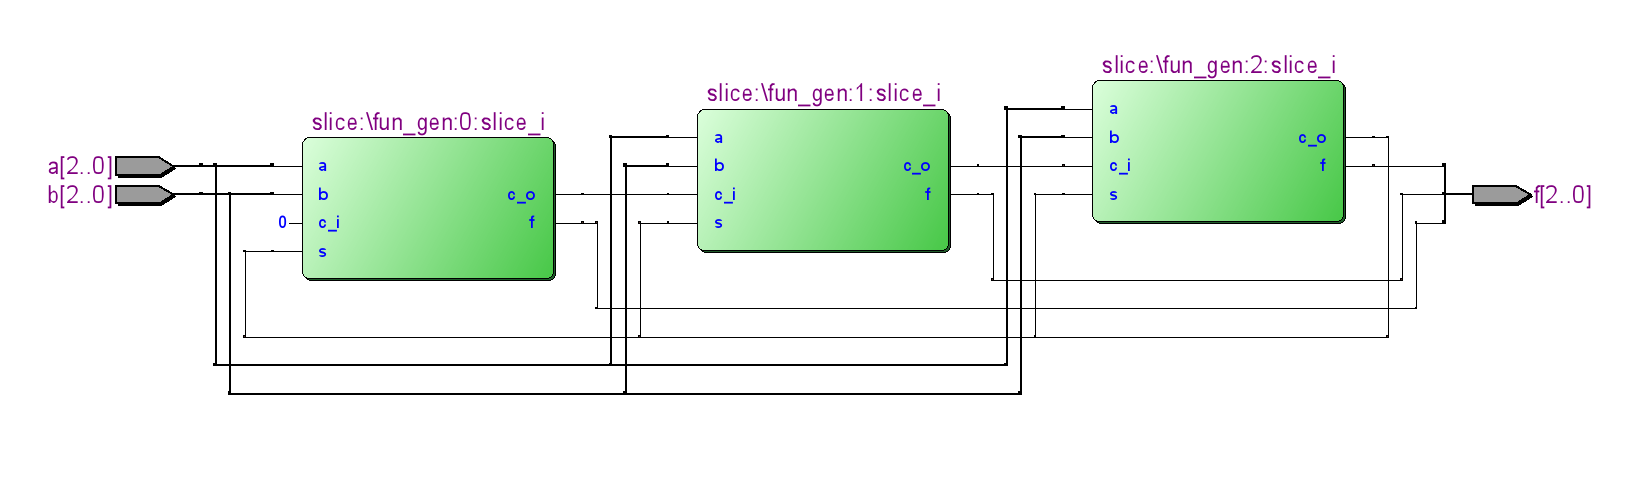
\includegraphics[width=\linewidth]{../part_2/fun_3_rtl.png}
    \caption{RTL block diagram of generated slices}
\end{figure}

\newpage
Once we verified that our generate block was correct we ran it through the same
simulations from Parts 1\&2. Both simulations completed successfully and spot
checks of the resulting waveforms also confirmed correct functionality. Given
that we ran the exact same exhaustive testbench as Parts 1\&2 we can say with
certainty that our sliced design is functionally equivalent.

\vspace{0.25in}
\begin{figure}[H]
    \centering
    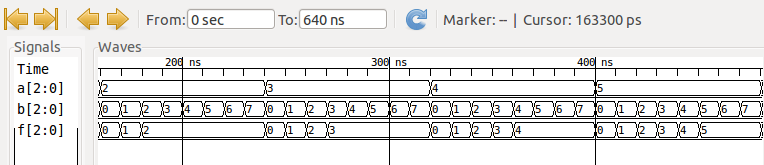
\includegraphics[width=\linewidth]{../part_2/fun_3.png}
    \caption{3-Bit FUN Generator}
\end{figure}
\vspace{0.25in}
\begin{figure}[H]
    \centering
    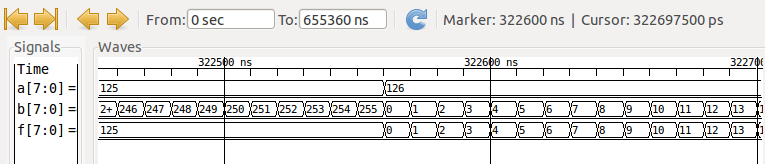
\includegraphics[width=\linewidth]{../part_2/fun_8.png}
    \caption{8-Bit FUN Generator}
\end{figure}

\newpage
\subsection*{Part 3}

In this section we were required to each design a layout based on the slice
design from Part 2.  Since we already had a gate level representation of our
slice it was fairly easy to convert it to a full CMOS representation using
FETs. A diagram illustrating this representation is shown below with all
transistors labeled. The size of the every transistor for both designs is
tabulated below:

\begin{table}[H]
    \centering
    \begin{tabular}{lc}
        \toprule
        \textbf{Parameter} & \textbf{Size} \\
        \midrule
        length    & 0.6u \\
        n width   & 1.2u \\
        p width   & 1.2u \\
        \bottomrule
    \end{tabular}
    \caption{Transistor Dimensions}
\end{table}
\vspace{0.5in}
\begin{figure}[H]
    \centering
    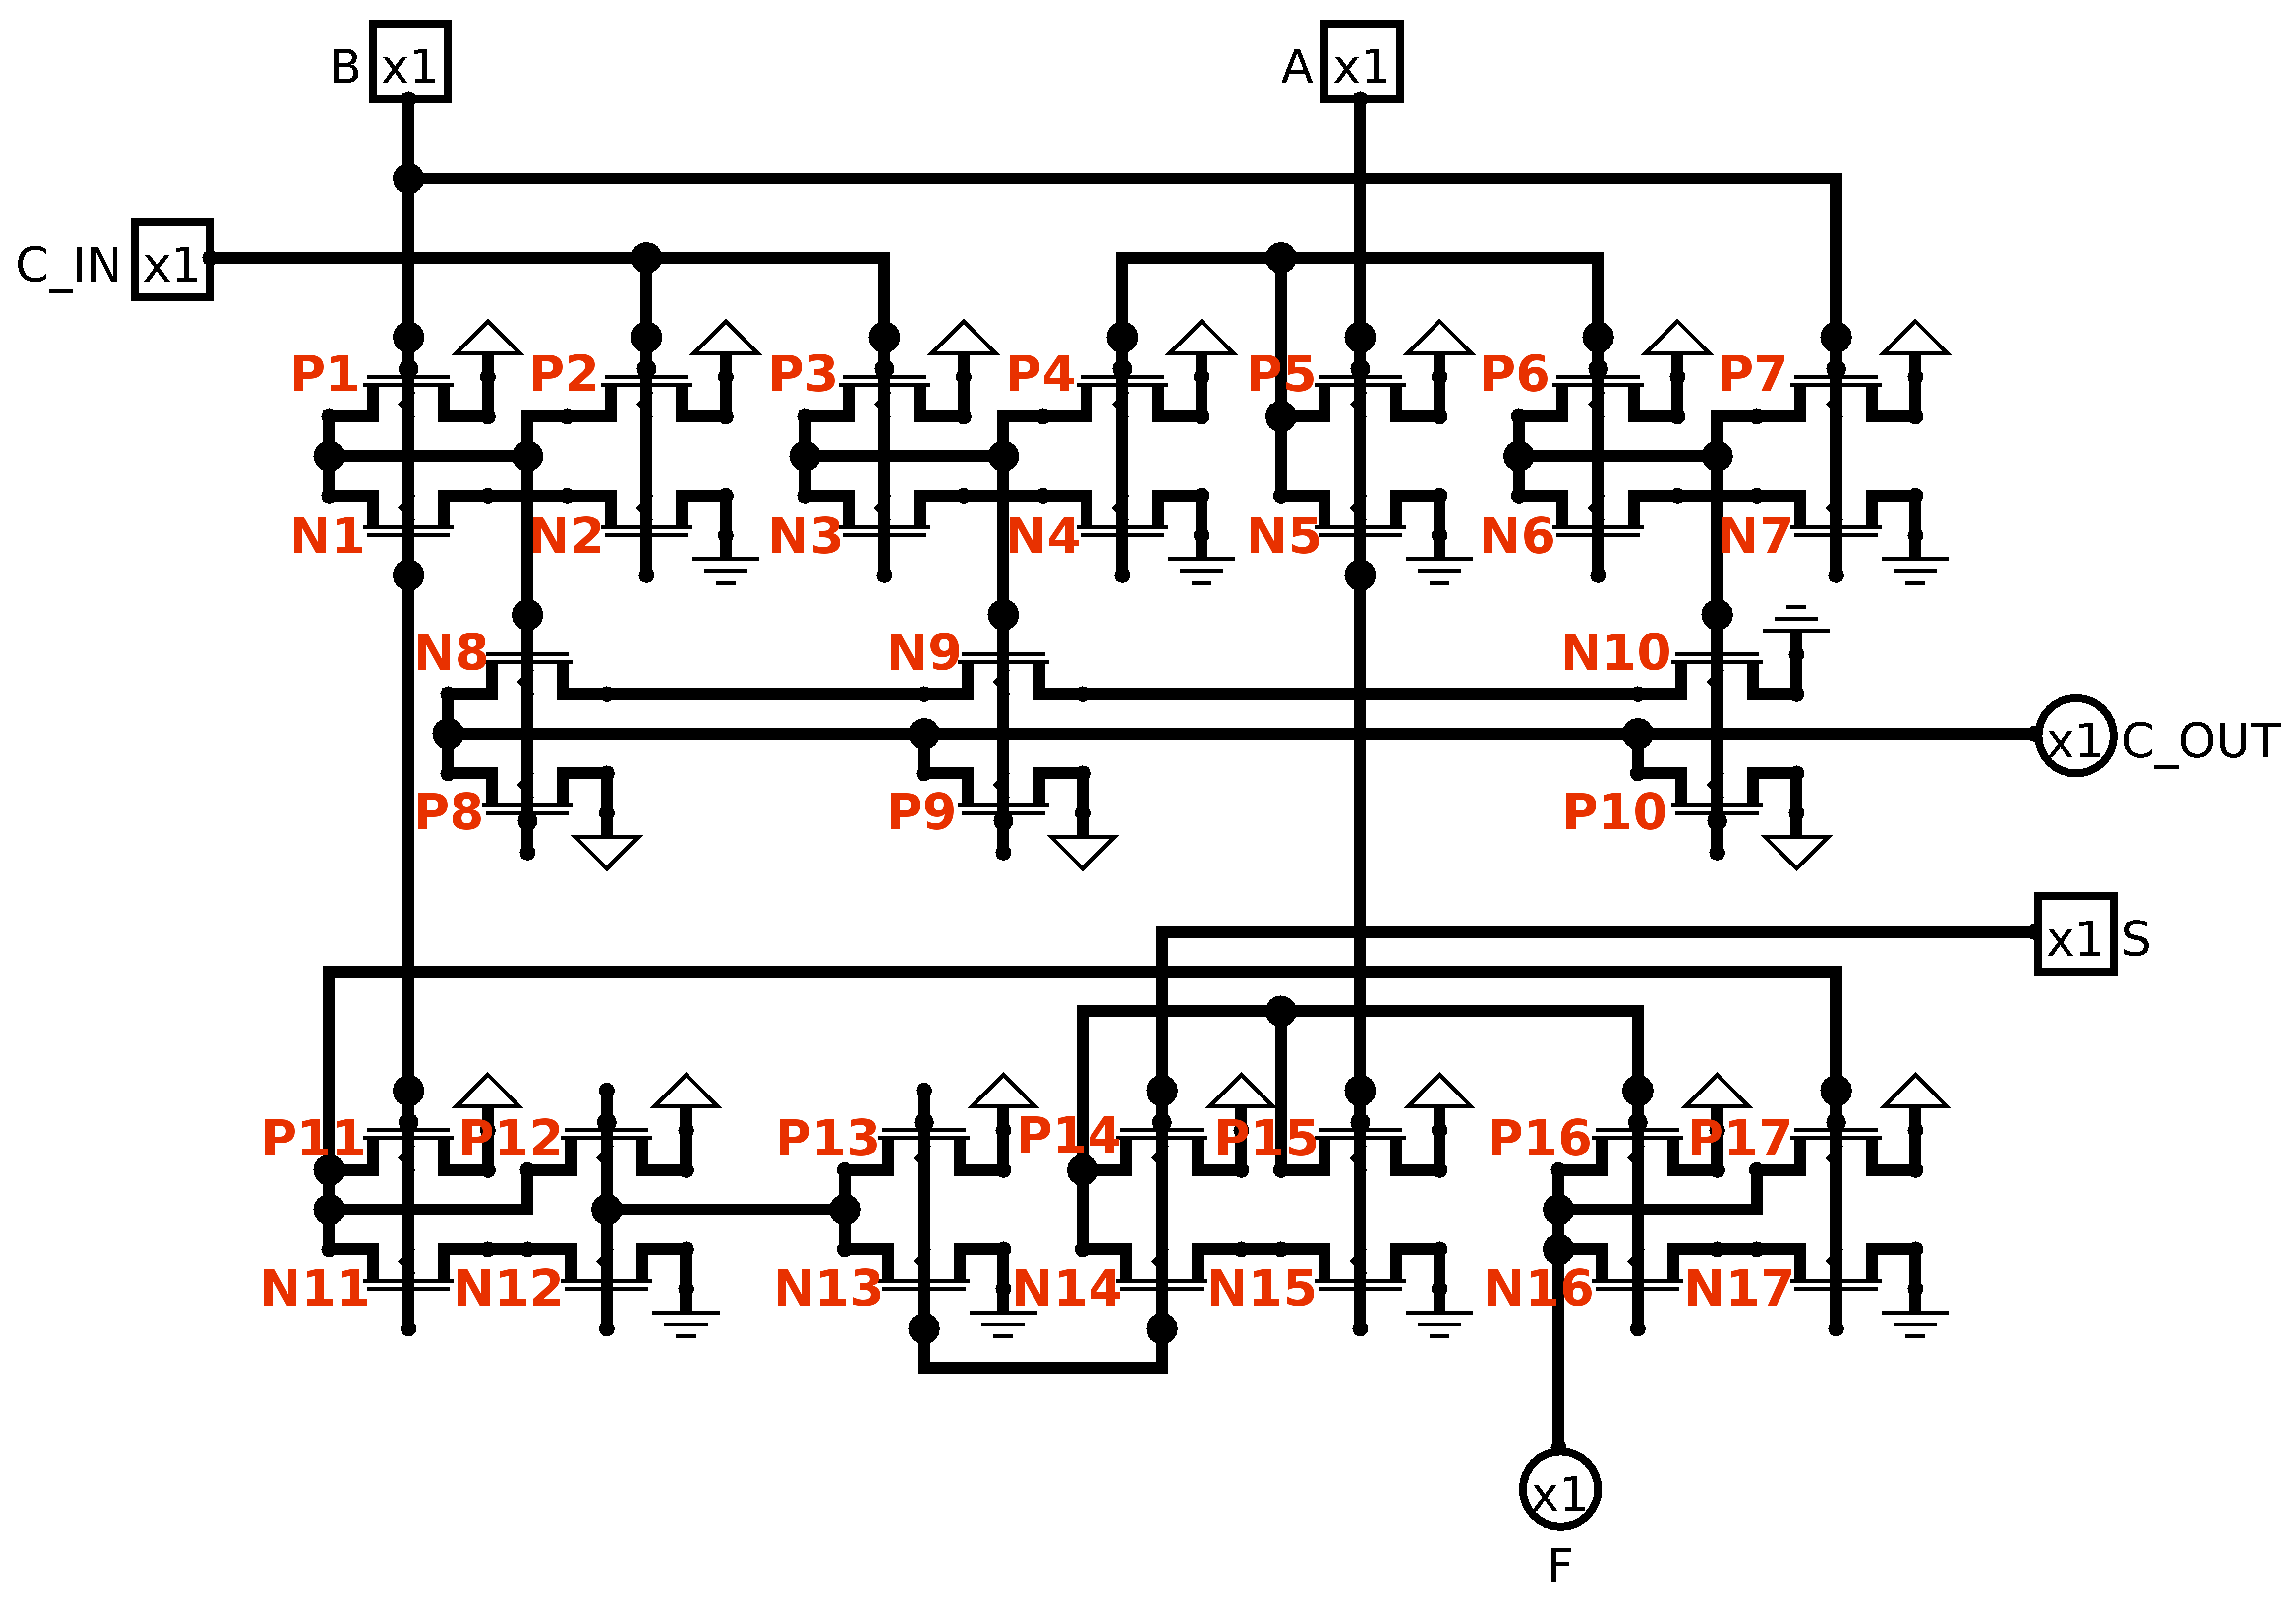
\includegraphics[width=\linewidth]{../logisim/logisim_bitslice_cmos_labeled.png}
    \caption{Transistor Diagram}
\end{figure}

\newpage
\subsubsection*{Design A (Qi)}

\begin{figure}[H]
    \centering
    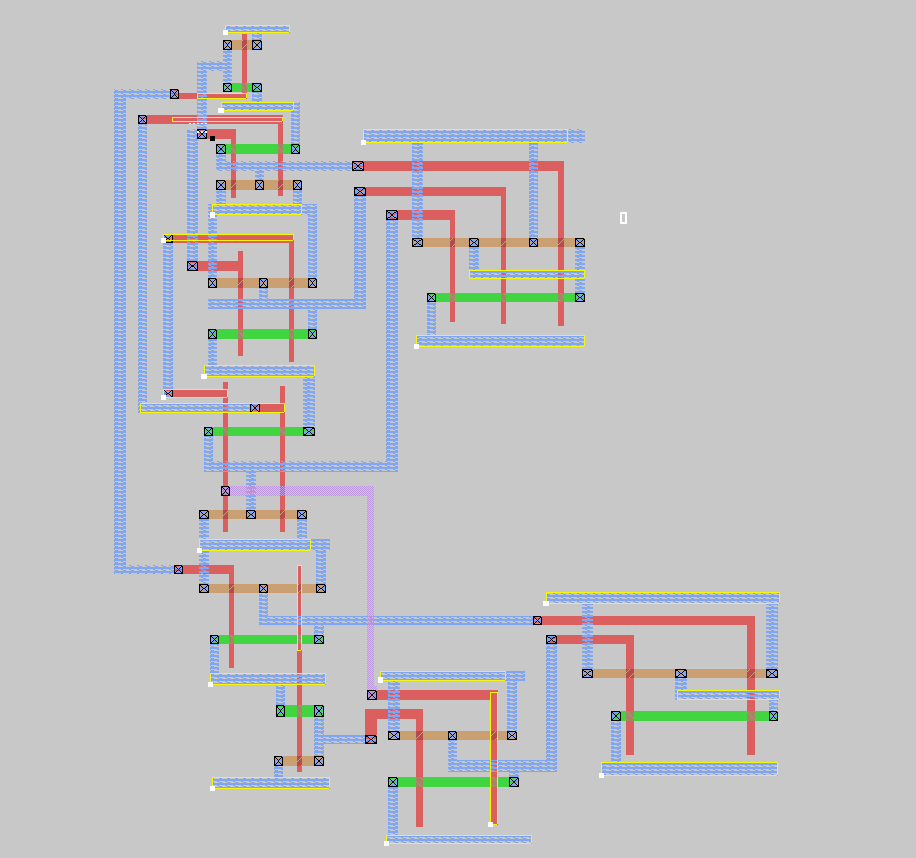
\includegraphics[width=\linewidth]{../part_3/xiaohui/magicslice.png}
    \caption{\textbf{Design A:} Layout}
\end{figure}

\newpage
\lstinputlisting[caption=\textbf{Design A:} IRSIM Command File]{../part_3/xiaohui/bitslice.cmd}

\begin{figure}[H]
    \centering
    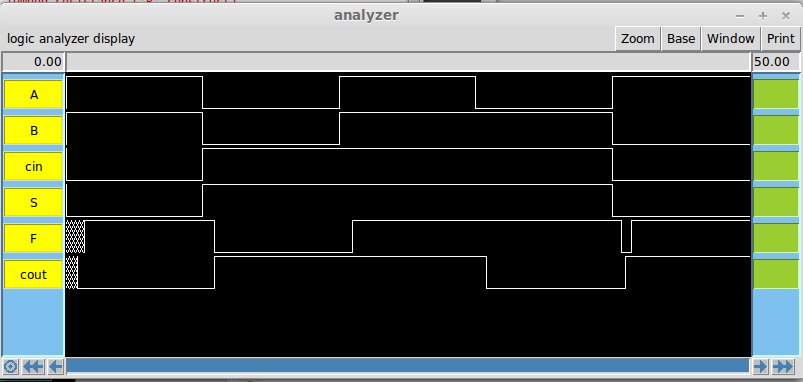
\includegraphics[width=\linewidth]{../part_3/xiaohui/irsimwaveform.png}
    \caption{\textbf{Design A:} IRSIM Output}
\end{figure}

\lstinputlisting[caption=\textbf{Design A:} Spice Simulation File]{../part_3/xiaohui/bitslice.sp}

\begin{figure}[H]
    \centering
    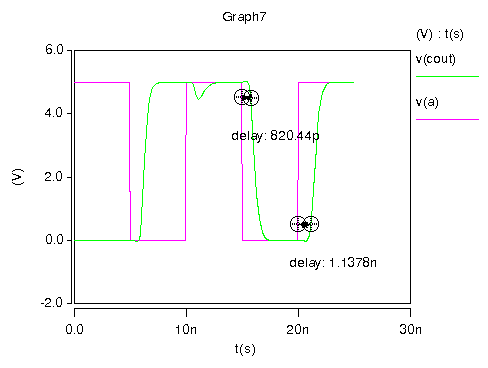
\includegraphics[height=4in]{../part_3/xiaohui/va_cout_delay_inv.png}
    \caption{\textbf{Design A:} A to C\_OUT Delay}
\end{figure}

\begin{figure}[H]
    \centering
    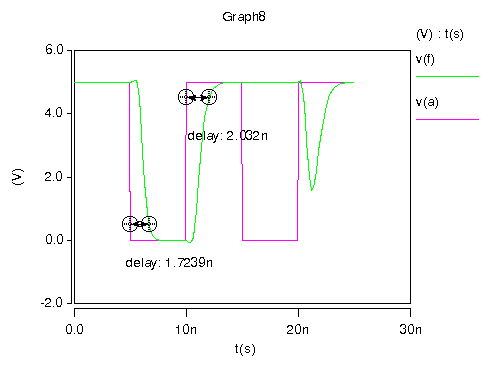
\includegraphics[height=4in]{../part_3/xiaohui/va_vf_delay_inv.png}
    \caption{\textbf{Design A:} A to F Delay}
\end{figure}

\newpage
\subsubsection*{Design B (Thrun)}

\begin{figure}[H]
    \centering
    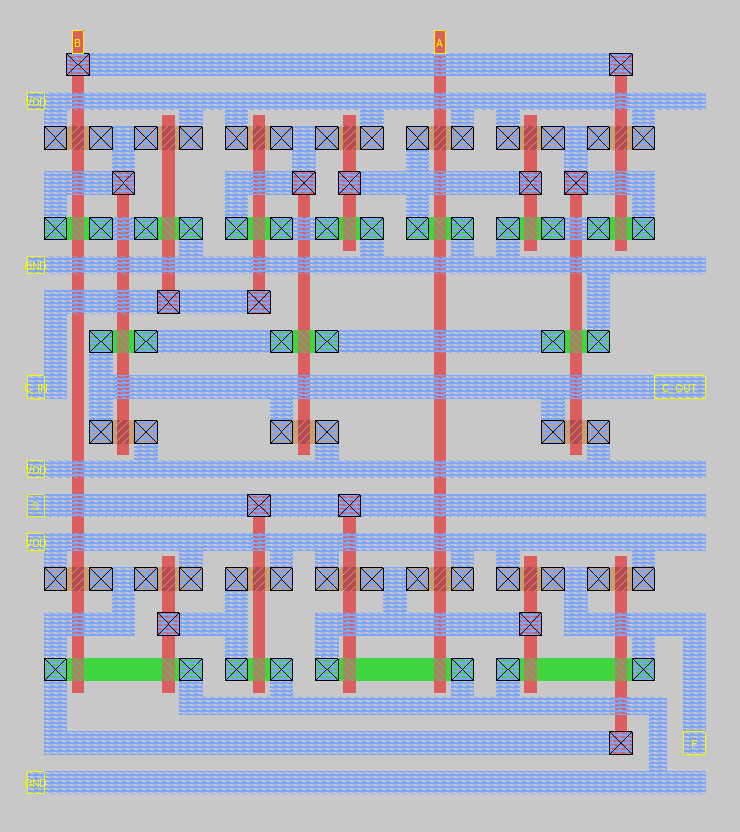
\includegraphics[width=\linewidth]{../part_3/max/max_layout.png}
    \caption{\textbf{Design B:} Layout}
\end{figure}

\newpage
\lstinputlisting[caption=\textbf{Design B:} IRSIM Command File (truncated), lastline=20]{../part_3/max/f.cmd}

\begin{figure}[H]
    \centering
    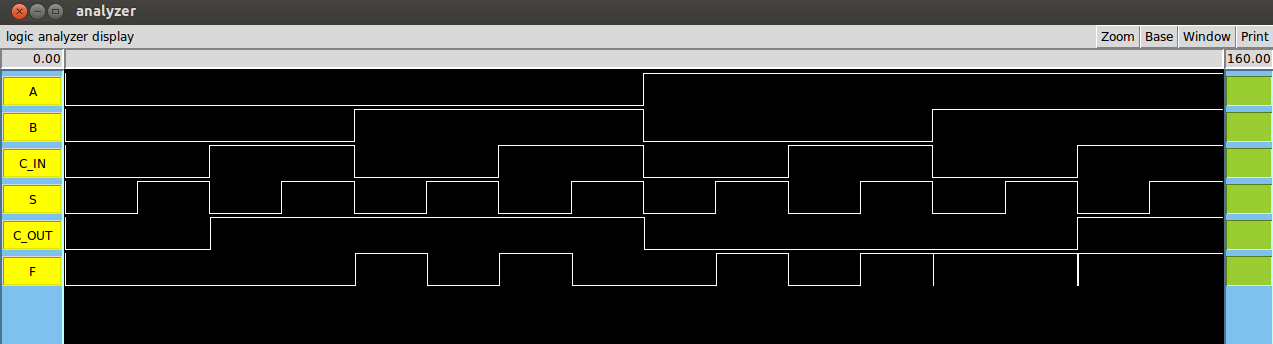
\includegraphics[width=\linewidth]{../part_3/max/max_irsim_glitch.png}
    \caption{\textbf{Design B:} IRSIM Output}
\end{figure}

\lstinputlisting[caption=\textbf{Design B:} Spice Simulation File]{../part_3/max/slice.sp}

\begin{figure}[H]
    \centering
    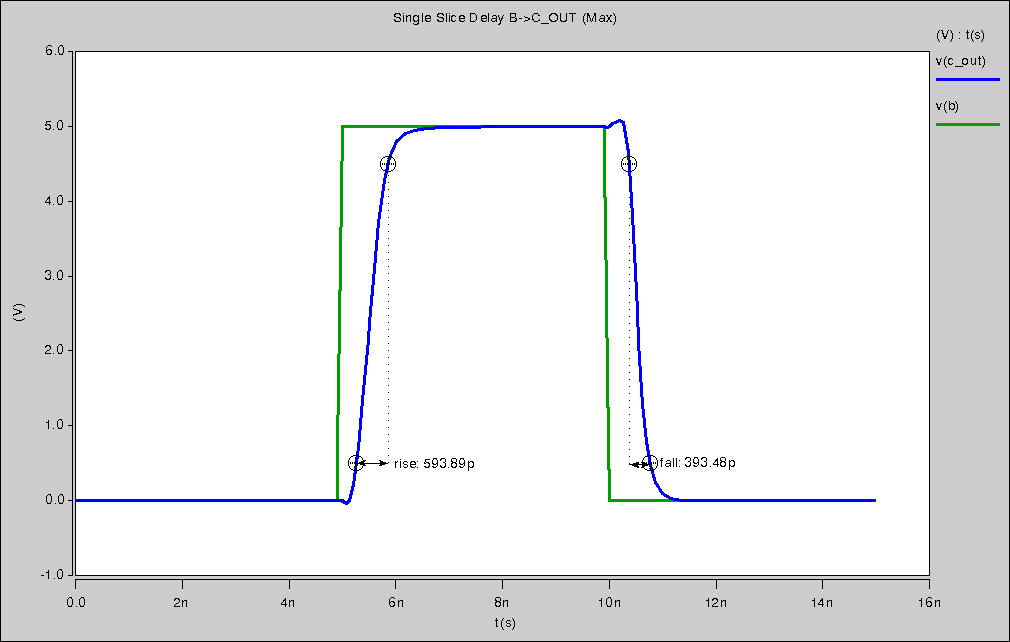
\includegraphics[width=\linewidth]{../part_3/max/max_single_slice_b_to_cout.png}
    \caption{\textbf{Design B:} B to C\_OUT Delay}
\end{figure}

\begin{figure}[H]
    \centering
    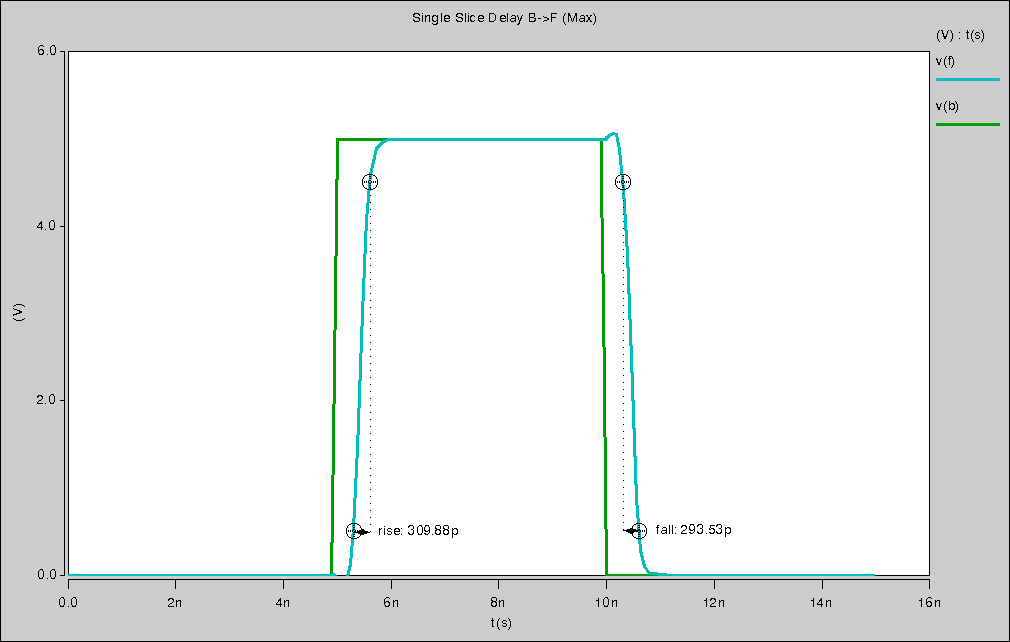
\includegraphics[width=\linewidth]{../part_3/max/max_single_slice_b_to_f.png}
    \caption{\textbf{Design B:} B to F Delay}
\end{figure}

\vspace{0.5in}
\subsubsection*{Design Summary}

A comparison of delays obtained from hspice for both designs is tabulated
below. From the results we can see that design B is significantly faster. Given
this result, combined with the fact that the layout of design B lends itself to
easier patterning, we chose design B as the design to move forward with.

\vspace{0.25in}
\begin{table}[H]
    \centering
    \begin{tabular}{lcc}
        \toprule
        \textbf{Parameter} & \textbf{Design A} & \textbf{Design B} \\
        \midrule
        A/B to C\_Out (Fall) & 820.44ps & 393.48ps \\
        A/B to C\_Out (Rise) & 1.1378ns & 593.89ps \\
        A/B to F (Fall)     & 1.7239ns & 293.53ps \\
        A/B to F (Rise)     & 2.0320ns & 309.88ps \\
        \bottomrule
    \end{tabular}
    \caption{Delay Comparison}
\end{table}

\newpage
\subsection*{Part 4}

The objective of this part was to rewrite our slice architecture from Part 2 to
use component instances of VHDL models of the static gates we used to implement
the slice ensuring that we include the worst case delay. In order to achieve this
the first thing we needed to do was simulate each gate and find the worst case delay
times. The spice simulation file and the resulting output for each of the three different
gates are shown below.

\begin{figure}[H]
    \centering
    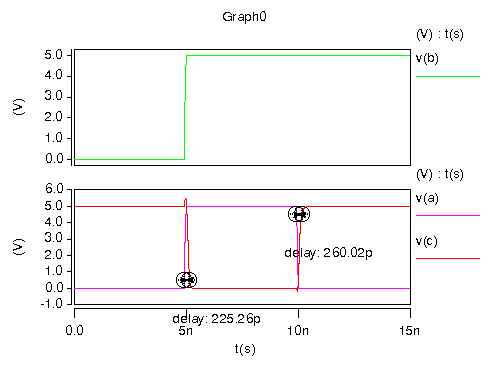
\includegraphics[width=0.75\linewidth]{../part_4/hspice/nand2_inv.png}
    \caption{2 Input NAND Gate}
\end{figure}

\lstinputlisting[caption=2 Input NAND Gate Spice Simulation File]{../part_4/hspice/nand2.sp}

\begin{figure}[H]
    \centering
    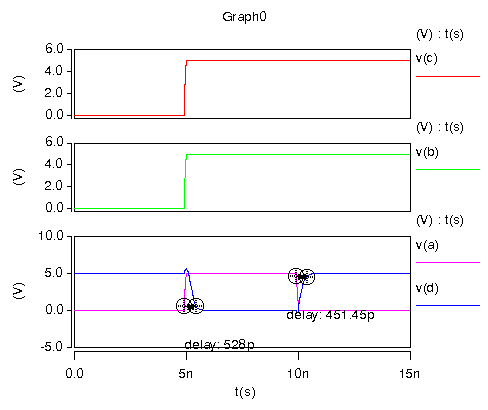
\includegraphics[width=0.75\linewidth]{../part_4/hspice/nand3_inv.png}
    \caption{3 Input NAND Gate}
\end{figure}

\lstinputlisting[caption=3 Input NAND Gate Spice Simulation File]{../part_4/hspice/nand3.sp}

\begin{figure}[H]
    \centering
    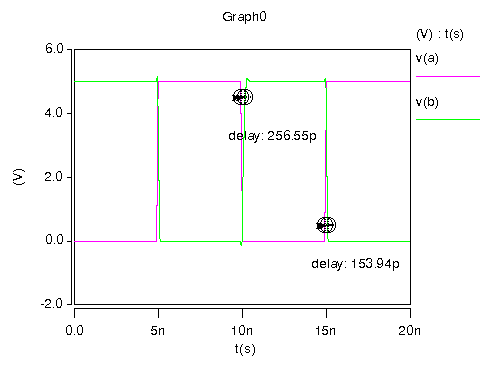
\includegraphics[width=0.75\linewidth]{../part_4/hspice/not_inv.png}
    \caption{NOT Gate}
\end{figure}

\lstinputlisting[caption=NOT Gate Spice Simulation File]{../part_4/hspice/not.sp}

\vspace{0.25in}
The worst case delays for each of these gates is tabulated below.

\begin{table}[H]
    \centering
    \begin{tabular}{lc}
        \toprule
        \textbf{Gate} & \textbf{Worst Case Delay} \\
        \midrule
        NAND-2 & 260.02ps \\
        NAND-3 & 528ps \\
        NOT    & 256.55ps \\
        \bottomrule
    \end{tabular}
    \caption{Worst Case Gate Delay}
\end{table}

\newpage
Knowing the worst case delay for each gate we can construct each as a separate module in VHDL.

\lstinputlisting[caption=2 Input NAND Gate Spice Simulation File]{../part_4/nandgate2.vhd}
\lstinputlisting[caption=3 Input NAND Gate Spice Simulation File]{../part_4/nandgate3.vhd}
\lstinputlisting[caption=NOT Gate Spice Simulation File]{../part_4/notgate.vhd}

With each gate implemented we can rewrite our slice to match the original gate
level design shown in part 2. The new slice module is shown below. Note that
the FUN module remains the same as Part 2.

\lstinputlisting[caption=Slice With Static Gates]{../part_4/slice.vhd}

\newpage
In our design the worst case delay is when a change in either A0 or B0 results in a change
in F0. The change in A0 or B0 has to propagate through all the slices and then back through
all the muxes until it finally reaches F0. Knowing this we can target our testbench to only
simulate this condition. The testbench simulating a 3-bit configuration is shown below. Note
that the testbench for the 8-bit configuration is exactly the same except the \texttt{n} constant
is changed to 8 and the input vectors are also 8 bit.

\lstinputlisting[caption=Static Gate Slice Testbench]{../part_4/fun_3_tb.vhd}

Looking at the output waveform we can measure the delta between the input state
change and the output state change. Measurements were taken for both a falling
edge and rising edge change for both the 3 and 8 bit configurations. The four
output waveforms are shown below.

\begin{figure}[H]
    \centering
    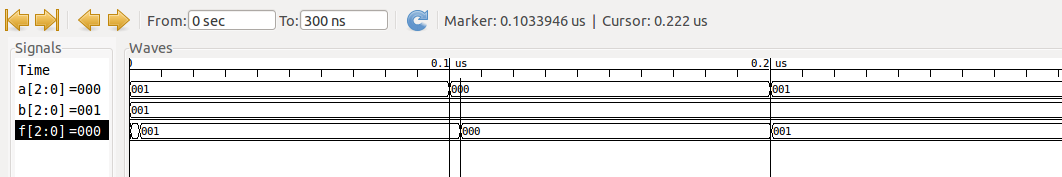
\includegraphics[width=\linewidth]{../part_4/fun_3_fall.png}
    \caption{3-Bit Fall Delay}
\end{figure}

\begin{figure}[H]
    \centering
    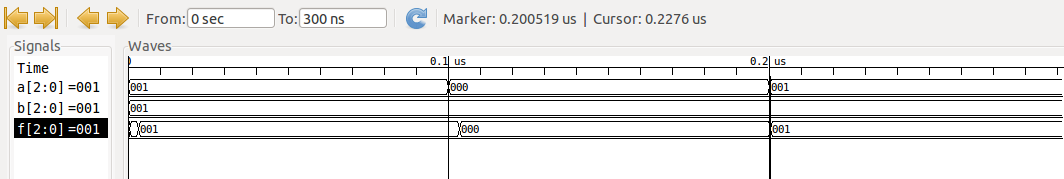
\includegraphics[width=\linewidth]{../part_4/fun_3_rise.png}
    \caption{3-Bit Rise Delay}
\end{figure}

\begin{figure}[H]
    \centering
    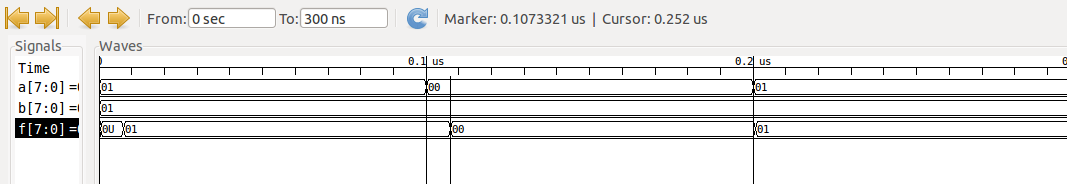
\includegraphics[width=\linewidth]{../part_4/fun_8_fall.png}
    \caption{8-Bit Fall Delay}
\end{figure}

\begin{figure}[H]
    \centering
    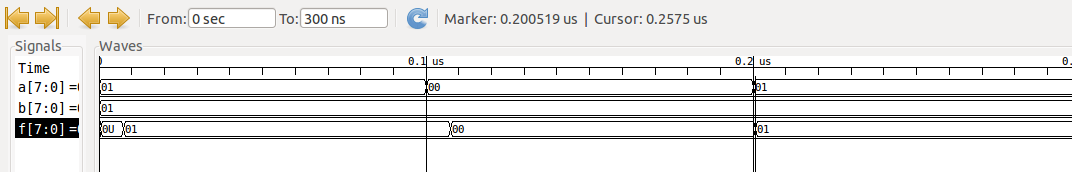
\includegraphics[width=\linewidth]{../part_4/fun_8_rise.png}
    \caption{8-Bit Rise Delay}
\end{figure}

\vspace{0.25in}
All the delays are tabulated below.

\begin{table}[H]
    \centering
    \begin{tabular}{ccc}
        \toprule
        \textbf{Configuration} & \textbf{Fall Delay} & \textbf{Rise Delay}\\
        \midrule
        3-Bit & 3.3946ns & 0.519ns \\
        8-Bit & 7.3321ns & 0.519ns \\
        \bottomrule
    \end{tabular}
    \caption{Worst Case Delay Through Chain}
\end{table}

\newpage
\subsection*{Part 5}

The objective of this section is to generate the layouts of a 3-bit and 8-bit
FUN generator and determine their worst case delays. This was easily achieved
by using the \texttt{array} command in magic. Since our slice tiles together
perfect it was almost trivial to chain them. The only paint we had to add was
to connect the last slices C\_OUT to the last slices S. The layouts for both
configurations are shown below.

\begin{figure}[H]
    \centering
    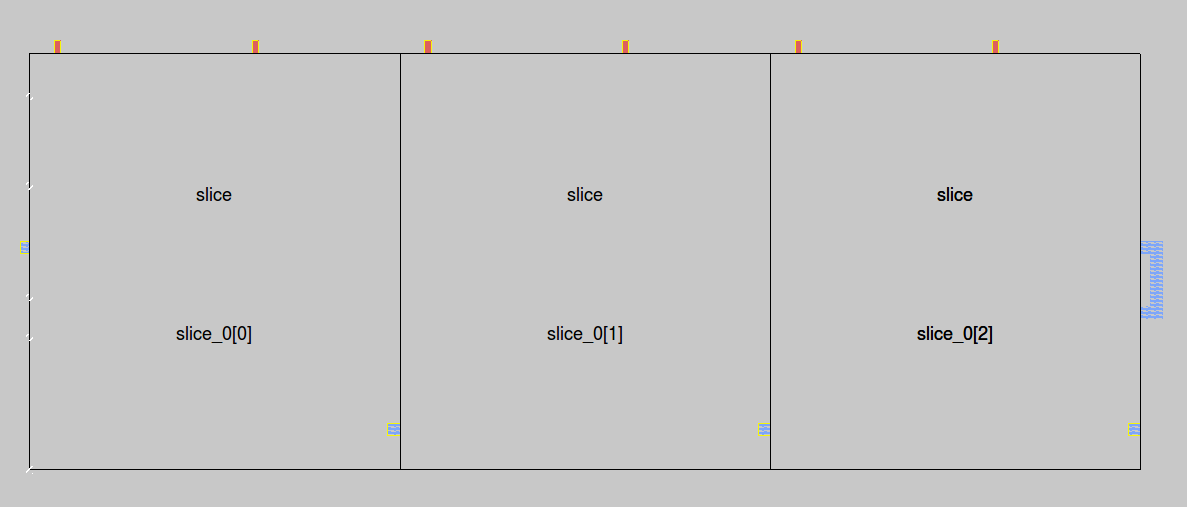
\includegraphics[width=\linewidth]{../part_5/fun_3_slices.png}
    \caption{3-Bit Layout}
\end{figure}

\begin{figure}[H]
    \centering
    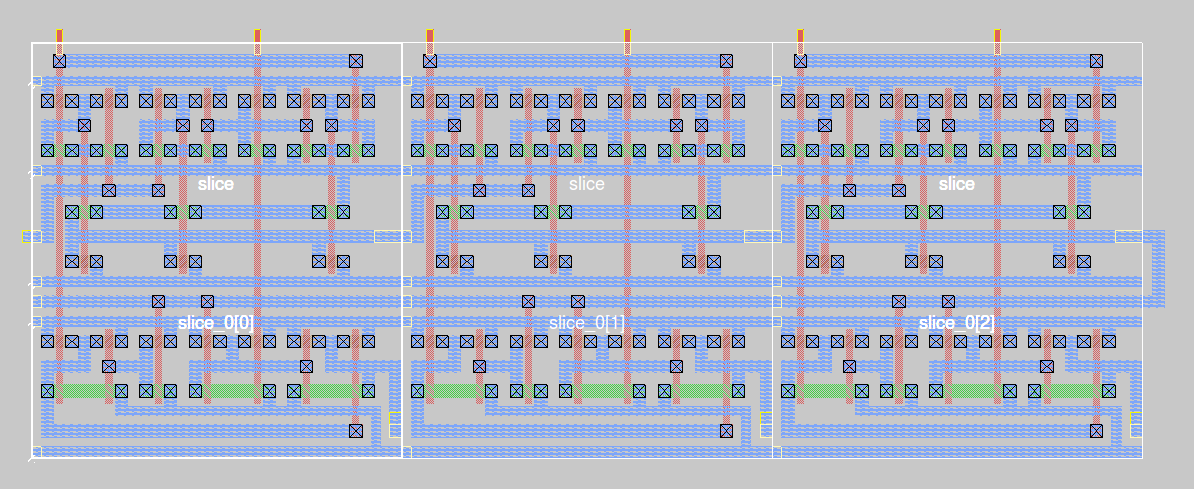
\includegraphics[width=\linewidth]{../part_5/fun_3_slices_full.png}
    \caption{3-Bit Layout Expanded}
\end{figure}

\newpage
\begin{figure}[H]
    \centering
    \begin{minipage}[t]{.5\textwidth}
        \centering
        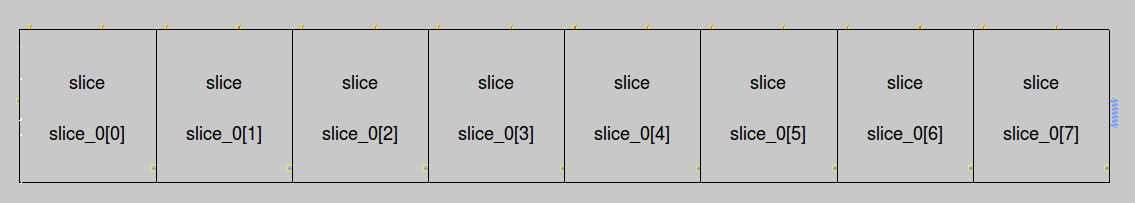
\includegraphics[width=9in, angle=270]{../part_5/fun_8_slices.png}
        \captionof{figure}{8-Bit Layout}
    \end{minipage}%
    \begin{minipage}[t]{.5\textwidth}
        \centering
        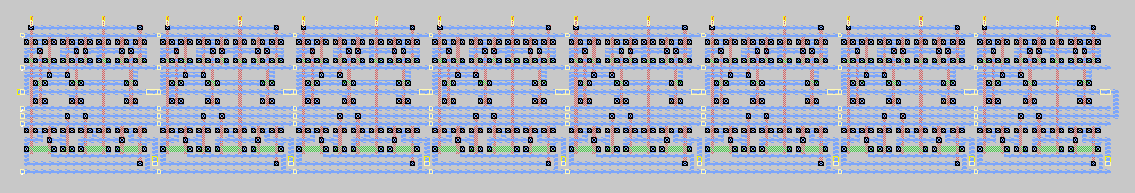
\includegraphics[width=9in, angle=270]{../part_5/fun_8_full.png}
        \captionof{figure}{8-Bit Layout Expanded}
    \end{minipage}%
\end{figure}

\newpage
In order to test the functionality of our multi-bit FUN generators we used two different
strategies. For the 3-bit version we simply did an exhaustive simulation and manually
looked at the waveform. To generate all the input vectors a simple Python script was
written. For the 8-bit version a similar strategy was used except instead of a completely
exhaustive search we skip over chunks.

\lstinputlisting[caption=Python Vector Generator, language=Python]{../part_5/gen_3.py}

The output IRSIM waveforms for each configuration is shown below.

\begin{figure}[H]
    \centering
    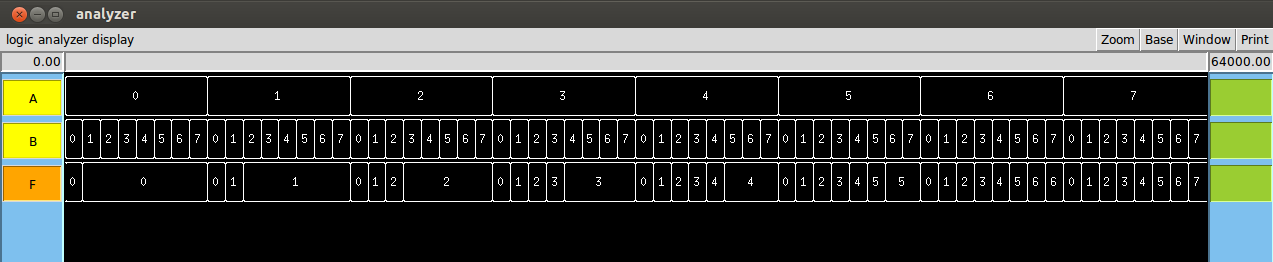
\includegraphics[width=\linewidth]{../part_5/irsim_3.png}
    \caption{3-Bit IRSIM Waveform}
\end{figure}

\begin{figure}[H]

    \centering
    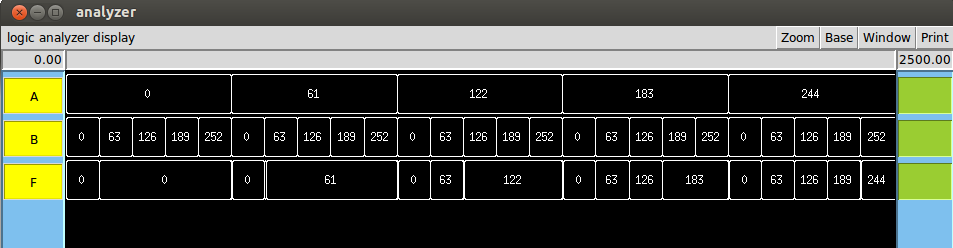
\includegraphics[width=\linewidth]{../part_5/irsim_8.png}
    \caption{8-Bit IRSIM Waveform}
\end{figure}

\vspace{0.125in}
To get the worst case delay out of IRSIM we utilized the \texttt{PATH} command
which tells you delay through the critical path. Interestingly it reported that
our worst case delay was \textbf{0.003ns} for each configuration. This is hard
to believe but it might be possible due to the fact that IRSIM says it's
`Ignoring lumped-resistance'. In regards to trying to increase the accuracy of
the VHDL model it could be possible to account for additional capacitances
introduced by the wiring of all the gates. Instead of introducing the delay per
gate you could introduce the total delay per slice. A table comparing these
results to the VHDL simulation is shown below.

\begin{table}[H]
    \centering
    \begin{tabular}{ccc}
        \toprule
        \textbf{Configuration} & \textbf{VHDL} & \textbf{IRSIM} \\
        \midrule
        3-Bit & 3.3946ns & 0.0030ns \\
        8-Bit & 7.3321ns & 0.0030ns \\
        \bottomrule
    \end{tabular}
    \caption{Worst Case Delay Comparison Between VHDL, IRSIM, and Spice}
\end{table}

\subsection*{Part 6}

The objective of this part was to simulate the layout level designs using
Spice. Since we only wanted to focus on the worst case delay we chose an input
transition on slice 0 that causes and output transition on slice 0. The
simulation file to achieve this is shown below. Note that the simulation file
for the 8-bit version is exactly the same except 5 more inputs are added, all
pulled to ground.

\vspace{0.25in}
\lstinputlisting[caption=3-Bit FUN Generator Spice Simulation]{../part_6/fun_3.sp}

\newpage
The output from both simulations is shown below

\begin{figure}[H]
    \centering
    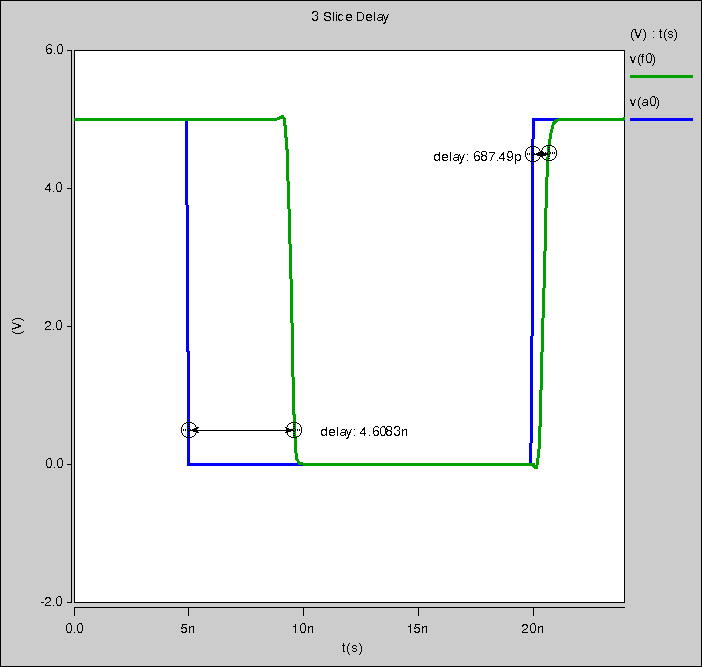
\includegraphics[width=0.6\linewidth]{../part_6/fun3.png}
    \caption{3-Bit Spice Waveform}
\end{figure}

\begin{figure}[H]
    \centering
    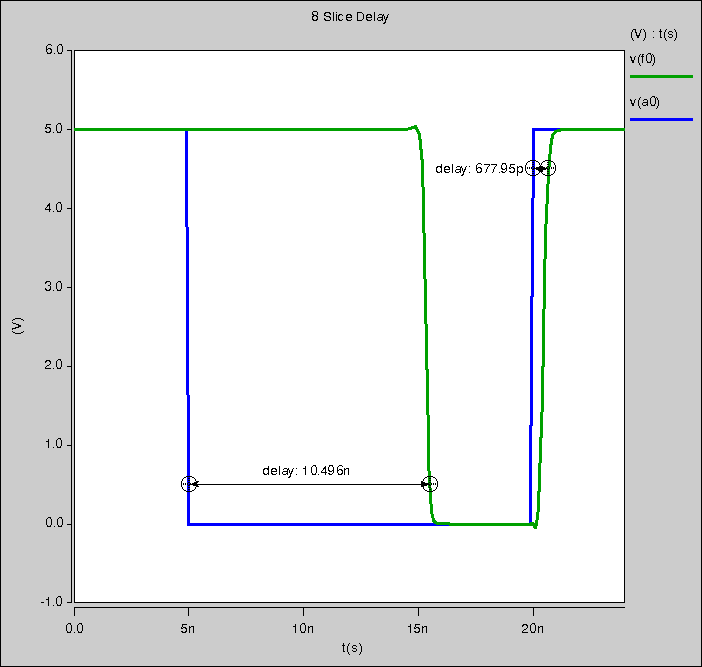
\includegraphics[width=0.6\linewidth]{../part_6/fun8.png}
    \caption{8-Bit Spice Waveform}
\end{figure}

\newpage
From the results we can see that our designs do seem to work correctly. Looking
at a final comparison of all the delays between VHDL, IRSIM, and Spice we can
clearly see that the VHDL simulation and Spice simulation are in agreement. The
IRSIM simulation results are unfortunately not in line with the other two
simulations.  This leads us to believe that our method of obtaining the worst
case delay with IRSIM is incorrect.

\vspace{0.25in}
\begin{table}[H]
    \centering
    \begin{tabular}{cccc}
        \toprule
        \textbf{Configuration} & \textbf{VHDL} & \textbf{IRSIM} & \textbf{Spice}\\
        \midrule
        3-Bit & 3.3946ns & 0.0030ns & 4.6083ns\\
        8-Bit & 7.3321ns & 0.0030ns & 10.496ns\\
        \bottomrule
    \end{tabular}
    \caption{Worst Case Delay Comparison Between VHDL, IRSIM, and Spice}
\end{table}

\vspace{0.25in}
There are a few things we can take with us into future design processes. The
first of which is spending some time upfront to figure out why IRSIM does not
seem to report the correct delays. At the moment it seems that the easiest method
to obtain an accurate simulation of our design is to export the Spice netlist
from Magic of either an individual gate or a functional block such as a slice.
The spice simulation can be simple as we just want to know the worst case
delay.  Once we obtain the delay we can add it to our VHDL model. Using the
VHDL model provides much more flexibility in terms of functional testing as we
can totally automate the testbench as we did in this lab. Hopefully, with this
insight we will be able to accomplish future design tasks in a more efficient manner.

\vspace{0.5in}
\subsection*{Task Breakdown}

\begin{table}[H]
    \centering
    \begin{tabular}{cl}
        \toprule
        \textbf{Task} & \textbf{Person}\\
        \midrule
        Part 1 & Qi \\
        Part 2 & Thrun \\
        Part 3 & Both \\
        Part 4 & Qi \\
        Part 5 & Thrun \\
        Part 6 & Qi (with Thrun input on conclusion)\\
        \bottomrule
    \end{tabular}
    \caption{Task Assignment}
\end{table}

\end{document}
